\documentclass{article}
%%%%%%%%%%%%%%%%%%%%%%%%%%%%%%%%%%%%%%%%%
% Lachaise Assignment
% Structure Specification File
% Version 1.0 (26/6/2018)
%
% This template originates from:
% http://www.LaTeXTemplates.com
%
% Authors:
% Marion Lachaise & François Févotte
% Vel (vel@LaTeXTemplates.com)
%
% License:
% CC BY-NC-SA 3.0 (http://creativecommons.org/licenses/by-nc-sa/3.0/)
% 
%%%%%%%%%%%%%%%%%%%%%%%%%%%%%%%%%%%%%%%%%

%----------------------------------------------------------------------------------------
%	PACKAGES AND OTHER DOCUMENT CONFIGURATIONS
%----------------------------------------------------------------------------------------

\usepackage{amsmath,amsfonts,stmaryrd,amssymb} % Math packages

\usepackage{enumerate} % Custom item numbers for enumerations

\usepackage[ruled]{algorithm2e} % Algorithms

\usepackage[framemethod=tikz]{mdframed} % Allows defining custom boxed/framed environments

\usepackage{listings} % File listings, with syntax highlighting
\lstset{
	basicstyle=\ttfamily, % Typeset listings in monospace font
}

%----------------------------------------------------------------------------------------
%	DOCUMENT MARGINS
%----------------------------------------------------------------------------------------

\usepackage{geometry} % Required for adjusting page dimensions and margins

\geometry{
	paper=a4paper, % Paper size, change to letterpaper for US letter size
	top=2.5cm, % Top margin
	bottom=3cm, % Bottom margin
	left=2.5cm, % Left margin
	right=2.5cm, % Right margin
	headheight=14pt, % Header height
	footskip=1.5cm, % Space from the bottom margin to the baseline of the footer
	headsep=1.2cm, % Space from the top margin to the baseline of the header
	%showframe, % Uncomment to show how the type block is set on the page
}

%----------------------------------------------------------------------------------------
%	FONTS
%----------------------------------------------------------------------------------------

\usepackage[utf8]{inputenc} % Required for inputting international characters
\usepackage[T1]{fontenc} % Output font encoding for international characters

\usepackage{XCharter} % Use the XCharter fonts

%----------------------------------------------------------------------------------------
%	COMMAND LINE ENVIRONMENT
%----------------------------------------------------------------------------------------

% Usage:
% \begin{commandline}
%	\begin{verbatim}
%		$ ls
%		
%		Applications	Desktop	...
%	\end{verbatim}
% \end{commandline}

\mdfdefinestyle{commandline}{
	leftmargin=10pt,
	rightmargin=10pt,
	innerleftmargin=15pt,
	middlelinecolor=black!50!white,
	middlelinewidth=2pt,
	frametitlerule=false,
	backgroundcolor=black!5!white,
	frametitle={Command Line},
	frametitlefont={\normalfont\sffamily\color{white}\hspace{-1em}},
	frametitlebackgroundcolor=black!50!white,
	nobreak,
}

% Define a custom environment for command-line snapshots
\newenvironment{commandline}{
	\medskip
	\begin{mdframed}[style=commandline]
}{
	\end{mdframed}
	\medskip
}

%----------------------------------------------------------------------------------------
%	FILE CONTENTS ENVIRONMENT
%----------------------------------------------------------------------------------------

% Usage:
% \begin{file}[optional filename, defaults to "File"]
%	File contents, for example, with a listings environment
% \end{file}

\mdfdefinestyle{file}{
	innertopmargin=1.6\baselineskip,
	innerbottommargin=0.8\baselineskip,
	topline=false, bottomline=false,
	leftline=false, rightline=false,
	leftmargin=2cm,
	rightmargin=2cm,
	singleextra={%
		\draw[fill=black!10!white](P)++(0,-1.2em)rectangle(P-|O);
		\node[anchor=north west]
		at(P-|O){\ttfamily\mdfilename};
		%
		\def\l{3em}
		\draw(O-|P)++(-\l,0)--++(\l,\l)--(P)--(P-|O)--(O)--cycle;
		\draw(O-|P)++(-\l,0)--++(0,\l)--++(\l,0);
	},
	nobreak,
}

% Define a custom environment for file contents
\newenvironment{file}[1][File]{ % Set the default filename to "File"
	\medskip
	\newcommand{\mdfilename}{#1}
	\begin{mdframed}[style=file]
}{
	\end{mdframed}
	\medskip
}

%----------------------------------------------------------------------------------------
%	NUMBERED QUESTIONS ENVIRONMENT
%----------------------------------------------------------------------------------------

% Usage:
% \begin{question}[optional title]
%	Question contents
% \end{question}

\mdfdefinestyle{question}{
	innertopmargin=1.2\baselineskip,
	innerbottommargin=0.8\baselineskip,
	roundcorner=5pt,
	nobreak,
	singleextra={%
		\draw(P-|O)node[xshift=1em,anchor=west,fill=white,draw,rounded corners=5pt]{%
		Question \theQuestion\questionTitle};
	},
}

\newcounter{Question} % Stores the current question number that gets iterated with each new question

% Define a custom environment for numbered questions
\newenvironment{question}[1][\unskip]{
	\bigskip
	\stepcounter{Question}
	\newcommand{\questionTitle}{~#1}
	\begin{mdframed}[style=question]
}{
	\end{mdframed}
	\medskip
}

%----------------------------------------------------------------------------------------
%	WARNING TEXT ENVIRONMENT
%----------------------------------------------------------------------------------------

% Usage:
% \begin{warn}[optional title, defaults to "Warning:"]
%	Contents
% \end{warn}

\mdfdefinestyle{warning}{
	topline=false, bottomline=false,
	leftline=false, rightline=false,
	nobreak,
	singleextra={%
		\draw(P-|O)++(-0.5em,0)node(tmp1){};
		\draw(P-|O)++(0.5em,0)node(tmp2){};
		\fill[black,rotate around={45:(P-|O)}](tmp1)rectangle(tmp2);
		\node at(P-|O){\color{white}\scriptsize\bf !};
		\draw[very thick](P-|O)++(0,-1em)--(O);%--(O-|P);
	}
}

% Define a custom environment for warning text
\newenvironment{warn}[1][Warning:]{ % Set the default warning to "Warning:"
	\medskip
	\begin{mdframed}[style=warning]
		\noindent{\textbf{#1}}
}{
	\end{mdframed}
}

%----------------------------------------------------------------------------------------
%	INFORMATION ENVIRONMENT
%----------------------------------------------------------------------------------------

% Usage:
% \begin{info}[optional title, defaults to "Info:"]
% 	contents
% 	\end{info}

\mdfdefinestyle{info}{%
	topline=false, bottomline=false,
	leftline=false, rightline=false,
	nobreak,
	singleextra={%
		\fill[black](P-|O)circle[radius=0.4em];
		\node at(P-|O){\color{white}\scriptsize\bf i};
		\draw[very thick](P-|O)++(0,-0.8em)--(O);%--(O-|P);
	}
}

% Define a custom environment for information
\newenvironment{info}[1][Info:]{ % Set the default title to "Info:"
	\medskip
	\begin{mdframed}[style=info]
		\noindent{\textbf{#1}}
}{
	\end{mdframed}
}

\usepackage{biblatex}
\addbibresource{bib.bib}
\usepackage{amsmath,amsfonts,amssymb,amsthm}
\newcounter{dummy} 
\numberwithin{dummy}{section}
\newtheorem{theoremeT}[dummy]{Theorem}
\newtheorem{definitionT}{Definition}[section]
% Theorem box
\newmdenv[skipabove=7pt,
skipbelow=7pt,
backgroundcolor=black!5,
linecolor=gray,
innerleftmargin=5pt,
innerrightmargin=5pt,
innertopmargin=5pt,
leftmargin=0cm,
rightmargin=0cm,
innerbottommargin=5pt]{tBox}
% Definition box
\newmdenv[skipabove=7pt,
skipbelow=7pt,
rightline=false,
leftline=true,
topline=false,
bottomline=false,
linecolor=gray,
innerleftmargin=5pt,
innerrightmargin=5pt,
innertopmargin=0pt,
leftmargin=0cm,
rightmargin=0cm,
linewidth=4pt,
innerbottommargin=0pt]{dBox}	
% Creates an environment for each type of theorem and assigns it a theorem text style from the "Theorem Styles" section above and a colored box from above
\newenvironment{theorem}{\begin{tBox}\begin{theoremeT}}{\end{theoremeT}\end{tBox}}
\newenvironment{exercise}{\begin{eBox}\begin{exerciseT}}{\hfill{\color{ocre}\tiny\ensuremath{\blacksquare}}\end{exerciseT}\end{eBox}}				  
\newenvironment{definition}{\begin{dBox}\begin{definitionT}}{\end{definitionT}\end{dBox}}	
\newenvironment{example}{\begin{exampleT}}{\hfill{\tiny\ensuremath{\blacksquare}}\end{exampleT}}		
\newenvironment{corollary}{\begin{cBox}\begin{corollaryT}}{\end{corollaryT}\end{cBox}}	
\usepackage{hyperref}
\usepackage{color, colortbl}
\usepackage{wrapfig}
\definecolor{Gray}{gray}{0.9}
%----------------------------------------------------------------------------------------
%	ASSIGNMENT INFORMATION
%----------------------------------------------------------------------------------------
\title{Audio Declipping} % Title of the assignment
\author{Damoun Ayman \\ \href{https://github.com/damounayman/signal_processing}{\small Github repository}} % Author name and email address
\date{\today} % University, school and/or department name(s) and a date
%----------------------------------------------------------------------------------------
% local packages
\usepackage{algorithm2e}
\usepackage{xcolor}

%----------------------------------
% custom style commands
%----------------------------------
% variable style command
\newcommand{\xvar}[1]{\textsf{#1}}

% horizontal alignment command
\newcommand{\xvbox}[2]{\makebox[#1][l]{#2}}

%----------------------------------
% set algorithm2e styles
%----------------------------------
% change algorithm font size
\SetAlFnt{\footnotesize}

% change algorithm caption style
\newcommand{\xAlCapSty}[1]{\small\sffamily\bfseries\MakeUppercase{#1}}
\SetAlCapSty{xAlCapSty}

% comment style (algorithms)
\newcommand{\xCommentSty}[1]{\scriptsize\ttfamily\textcolor{blue}{#1}}
\SetCommentSty{xCommentSty}

% change line number style
\newcommand\mynlfont[1]{\scriptsize\sffamily{#1}}
\SetNlSty{mynlfont}{}{} 

 % add the line numbers
\LinesNumbered

% comments right justified
\SetSideCommentRight

% don't print semicolon
\DontPrintSemicolon

% ruled algorithm
\RestyleAlgo{algoruled}
\begin{document}
\maketitle % Print the title
%----------------------------------------------------------------------------------------
%	INTRODUCTION
%----------------------------------------------------------------------------------------
\section{Introduction}
Clipping or saturation is  common  distortions in  digital signal  processing. Cipping occurs when the signal reaches a maximum threshold and the waveform is truncated. In the literature there are several approaches to answer this issue: Can we get a good estimation of the original signal from the clipped one ?\\
In  this  report   we  address  the  problem  of recovering a signal from clipped measurements. Based on the methodology developed in the article \cite{inproceedings}.
\begin{figure}[ht!]
    \centering
    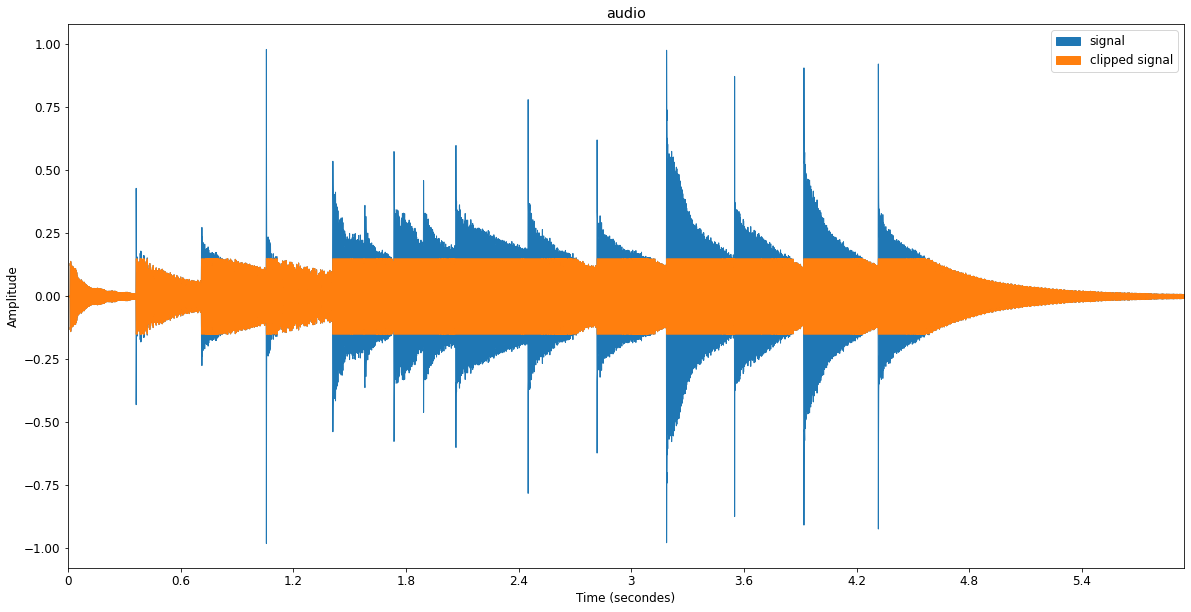
\includegraphics[scale=0.3]{figures/cvd.png}
    \caption{How to estimate the original signal (blue) from the clipped one (orange) ?}
    \label{reff}
\end{figure}
\section{Audio Declipping with Social Sparsity paper discuss}
The authors of the paper \cite{inproceedings} presents state of the art approach to recover clipped signal by using iterative thresholding algorithms and the principle of social sparsity.
\subsection{Background (Definitions)}
Let $s \in \mathbb{C}^N$ be the undistorted signal that we want to recover. Audio declipping can be formulated as :
\begin{equation}
\mathbf{y}^{r}=\mathbf{M}^{r} \mathbf{s}    
\label{equa1}
\end{equation}
$\mathbf{y}^{r} \in \mathbb{C}^{M}$ are the reliable sample of the observed signal\\
$\mathbf{M}^{r} \in \mathbb{C}^{M \times N}$ is the matrix of the reliable parts of $\mathbf{s}$\\
we apply a mask $M^r$ to the  sample signal to identifey the  reliable sample of the observed signal.\\
we can also define the clipped samples as:
\begin{equation}
\mathbf{y}^{m}=\mathbf{M}^{m} \mathbf{s}
\label{equa2}
\end{equation}
Both matrices $M^r$, $M^m$ are based on the skeleton of the identity matrix. they are  built  by  setting  the  corresponding  values  of  the identity matrix to 0 and do not reduce dimension.
\begin{figure}[ht!]
    \centering
    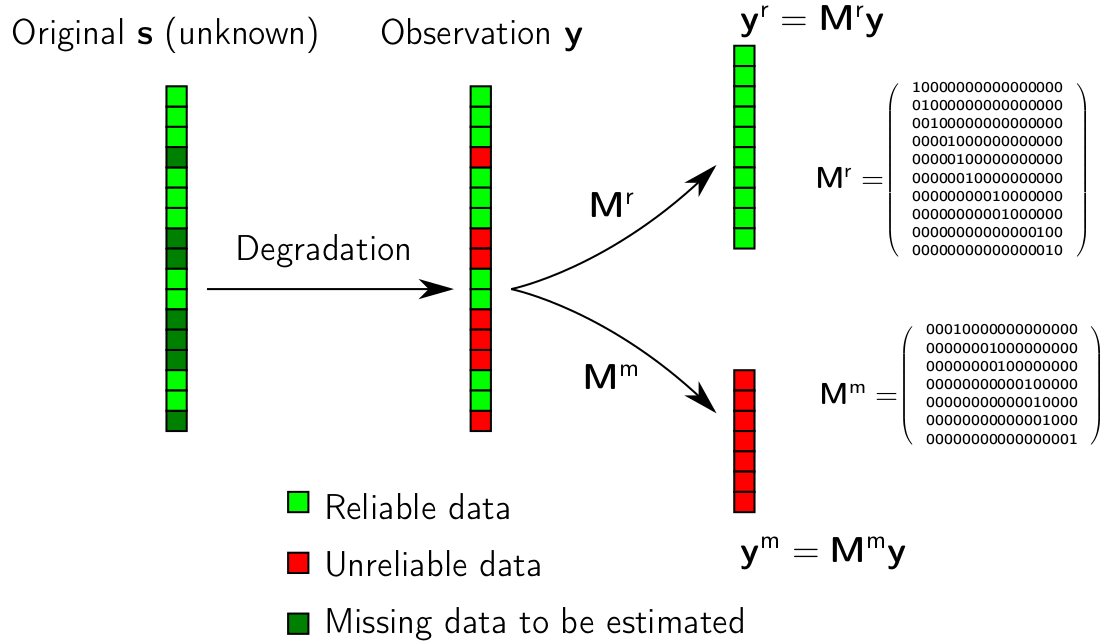
\includegraphics[scale=0.3]{figures/cd&&&&&&&&&&.png}
    \caption{Reliable and unreliable coefficient \cite{Matthieu} }
    \label{fig:my_label}
\end{figure}

For example, in dimension N= 4 with samples 2 and 4 distorted
$$
\boldsymbol{M}^{r}=\left[\begin{array}{cccc}
1 & 0 & 0 & 0 \\
0 & 0 & 0 & 0 \\
0 & 0 & 1 & 0 \\
0 & 0 & 0 & 0
\end{array}\right] \text { and } \; \boldsymbol{M}^{m}=\left[\begin{array}{cccc}
0 & 1 & 0 & 0 \\
0 & 0 & 0 & 1
\end{array}\right]
$$
It is clear that it is an undetermined problem. there is an infinity of possible estimation of $s$ that verifies the equation (\ref{equa1}) and (\ref{equa2}). To find a good solution, we need prior information about $s$. This information comes in the form the chosen model of the signal, which constrains the values of $s$. Sparse model can be used to address this problem.\\
\subsubsection{Sparse model}
A sparse model assume that a signal $s$ can be represented by summing up  few elementary pieces of signal, called atoms.\\
Formally:
$$
\mathbf{s}=\Phi \alpha
$$
with $\Phi \in \mathbb{C}^{M*N}$ is called the dictionnary of $\phi_k$ atoms and $\alpha \in \mathbb{C}^N$ is sparse.
\begin{figure}[ht!]
    \centering
    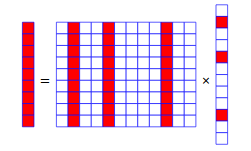
\includegraphics[scale=0.7]{figures/ls.png}
    \caption{Graphical representation of the sparse synthesis model \cite{gaultier:tel-02148598}}
    \label{fig:f}
\end{figure}
\begin{warn}[Note:]
A bad choice of dictionary will result in a bad modeling of the signal 
\end{warn}
\subsubsection{Inverse problem framework}
\begin{definition}
$$
\hat{\mathbf{s}}=\underset{\mathbf{s}}{\arg \min } \mathcal{L}(\mathbf{y}, A, \mathbf{s})+P(\mathbf{s} ; \lambda)
$$
With $\mathcal{L}(\mathbf{y}, A, \mathbf{s})$ convex loss or data term ,\\
A regularization term $P$ modeling the assumptions about the sources,\\
An hyperparameter $\lambda \in \mathbb{R}_{+}$
\end{definition}

\subsection{Problem formulation}
\subsubsection{Constrained and convex inverse problem}
Using the dictionnary $\Phi$ and sparsity.
the audio declipping problem can be formulate as constrained convex optimization problem.
\begin{equation}
\begin{aligned}
\hat{\boldsymbol{\alpha}}=& \underset{\boldsymbol{\alpha}}{\arg \min } \frac{1}{2}\left\|\mathbf{y}^{r}-\mathbf{M}^{r} \mathbf{\Phi} \boldsymbol{\alpha}\right\|+\lambda\|\boldsymbol{\alpha}\|_{1} \\
\text { s.t. } & \mathbf{M}^{m^{+}} \mathbf{\Phi} \boldsymbol{\alpha}>\theta^{\text {clip }} \\
& \mathbf{M}^{m^{-}} \mathbf{\Phi} \boldsymbol{\alpha}<-\theta^{\text {clip}}
\end{aligned}
\label{ref}
\end{equation}
where
$\mathbf{M}^{m^{+}}\left(\right.$ resp. $\left.\mathbf{M}^{m^{-}}\right.)$ select the positive (resp. negative) missing samples.\\
$\theta^{clip}$ is the clip threshold
\subsubsection{Rewrite the constraints}
The constrainted convex optimination problem \ref{ref} can be rewrited using the well-known function \textit{squared hinge} defined as follows:

$$
h^{2}: \mathbb{R} \longrightarrow \mathbb{R}_{+} \quad z \mapsto h^{2}(z)=\left\{\begin{array}{ll}
z^{2} & \text { if } z<0 \\
0 & \text { if } z \geq 0
\end{array}\right.
$$
By changing the variable $z=x-\theta^{clip}$\\
\[
\begin{cases}
\mathcal{L}\left(\theta^{\text {clip }}-x\right)=0, & \text{if $x\geq \theta^{c l i p}$} \\
\mathcal{L}\left(\theta^{\text {clip }}-x\right)=\left(\theta^{\text {clip }}-x\right)^{2}, & \text{if $x<\theta^{c l i p}$} 
\end{cases}
\]

Let
$$
\left[\boldsymbol{\theta}^{c l i p}-\mathbf{x}\right]_{+}^{2}=\sum_{k: \theta_{k}^{c l i p}>0}\left(\theta_{k}^{c l i p}-x_{k}\right)_{+}^{2}+\sum_{k: \theta_{k}^{c l i p}<0}\left(-\theta_{k}^{c l i p}+x_{k}\right)_{+}^{2}
$$
That leads to the following unconstrained convex problem:
\begin{equation}
\boldsymbol{\alpha}=\underset{\boldsymbol{\alpha}}{\arg \min } \frac{1}{2}\left\|\mathbf{y}^{r}-\mathbf{M}^{r} \boldsymbol{\Phi} \boldsymbol{\alpha}\right\|_{2}^{2}+\frac{1}{2}\left[\boldsymbol{\theta}^{c l i p}-\mathbf{M}^{m} \boldsymbol{\Phi} \boldsymbol{\alpha}\right]_{+}^{2}+ \lambda\|\boldsymbol{\alpha}\|_{1}
\label{equa}
\end{equation}
which is under the form
$$
f_{1}(\boldsymbol{\alpha})+f_{2}(\boldsymbol{\alpha})
$$
with $f_{1}$ Lipschitz-differentiable and $f_{2}$ semi-convex.\\
The  iterative shrinkage-thresholding algorithm (ISTA)  \cite{4959678} can be applied to solve the (\ref{equa}).\\
\subsection{Solution}
The social sparsity procedure allows shrinkage of a coefficient based on the values of coefficients in its  neighborhood.
The authors of the paper suggests using four types of social shrinkage of Time-frequency (TF) coefficients to approximate a solution to (\ref{equa}). Let $N(t)$ be the set of indices forming the neighborhood of the index t for the time-frequency coefficients $\alpha = \{\alpha_{tf}\}$.
\begin{itemize}
    \item \textbf{Lasso:} $$\tilde{\alpha}_{t f}=\mathbb{S}_{\lambda}^{L}\left(\alpha_{t f}\right)=\alpha_{t f}\left(1-\frac{\lambda}{\left|\alpha_{t f}\right|}\right)^{+}$$
    \item \textbf{WGL:} Windowed Group Lasso $$\tilde{\alpha}_{t f}=\mathbb{S}_{\lambda}^{W G L}\left(\alpha_{t f}\right)=\alpha_{t f}\left(1-\frac{\lambda}{\sqrt{\sum_{t^{\prime} \in \mathcal{N}(t)}\left|\alpha_{t^{\prime} f}\right|^{2}}}\right)^{+}$$
    \item \textbf{EW:} Empirical Wiener $$\tilde{\alpha}_{t f}=\mathbb{S}_{\lambda}^{E W}\left(\alpha_{t f}\right)=\alpha_{t f}\left(1-\frac{\lambda^{2}}{\left|\alpha_{t f}\right|^{2}}\right)^{+}$$
    \item \textbf{PEW:} Persistent Empirical Wiener $$\tilde{\alpha}_{t f}=\mathbb{S}_{\lambda}^{P E W}\left(\alpha_{t f}\right)=\alpha_{t f}\left(1-\frac{\lambda^{2}}{\sum_{t^{\prime} \in \mathcal{N}(t)}\left|\alpha_{t^{\prime} f}\right|^{2}}\right)^{+}$$
\end{itemize}
The ISTA Social sparsity declipper algorithm used in \cite{inproceedings} is presented below:
\begin{algorithm}

% functions
\SetKwFunction{cumprod}{cumprod}
\SetKwFunction{length}{length}
\SetKwFunction{zeros}{zeros}
\SetKwFunction{ceil}{ceil}

% input/ouput names
\SetKwInOut{Input}{Input}
\SetKwInOut{Output}{Output}

% caption
\caption{ISTA-type Social sparsity declipper \cite{inproceedings}\label{alg:singlepm}}

\Input{%
		\xvbox{2mm}{$\xvar{y}$} -- the observed signal \\
		$\delta=\left\|\boldsymbol{\Phi} \boldsymbol{\Phi}^{*}\right\|$\\
		$\boldsymbol{\alpha}^{(0)} \in \mathbb{C}^{N}$,$\lambda>0$\\
	  }
  \BlankLine % blank line for spacing
  
  % start of the pseudocode

  \xvbox{2mm}{$\mathbf{z}^{0}$} $\leftarrow$ $\boldsymbol{\alpha}^{(0)}$ \tcc*{Initialization}
        
  \For{$\xvar{i} = 1,...\textbf{until}$ convergence}{

    \xvbox{1mm}{$\xvar{g}_1$}\quad $\leftarrow$ $-\boldsymbol{\Phi}^{*} \mathbf{M}^{r^{T}}\left(\mathbf{y}^{r}-\mathbf{M}^{r} \mathbf{\Phi} \mathbf{z}^{(i-1)}\right)$ \tcc*{gradients}

    \xvbox{1mm}{$\xvar{g}_2$}\quad $\leftarrow$ $-\boldsymbol{\Phi}^{*} \mathbf{M}^{c^{T}}\left[\boldsymbol{\theta}^{c l i p}-\mathbf{M}^{c} \boldsymbol{\Phi} \mathbf{z}^{(i-1)}\right]_{+}$ 

    ${\alpha}^{i}$ $\leftarrow$ $\mathbb{S}_{\lambda / \delta}\left(\mathbf{z}^{(i-1)}-\frac{1}{\delta}(\mathbf{g} 1+\mathbf{g} 2)\right)$ \tcc*{step, shrink}

    $\mathbf{z}^{i}$ $\leftarrow$ $\boldsymbol{\alpha}^{(i)}+\gamma\left(\boldsymbol{\alpha}^{(i)}-\boldsymbol{\alpha}^{(i-1)}\right)$ \tcc*{extrapolate}
	
  } % end for j	
\textbf{return} $\Phi \alpha^{(i)}$
\end{algorithm}
For the choice of hyperparameter $\lambda$ a large value is chosen for a hundreds of iterations, then $\lambda$  is decreased until the target one.
\subsection{Numerical results}
\begin{wrapfigure}{r}{0.5\textwidth}
  \begin{center}
    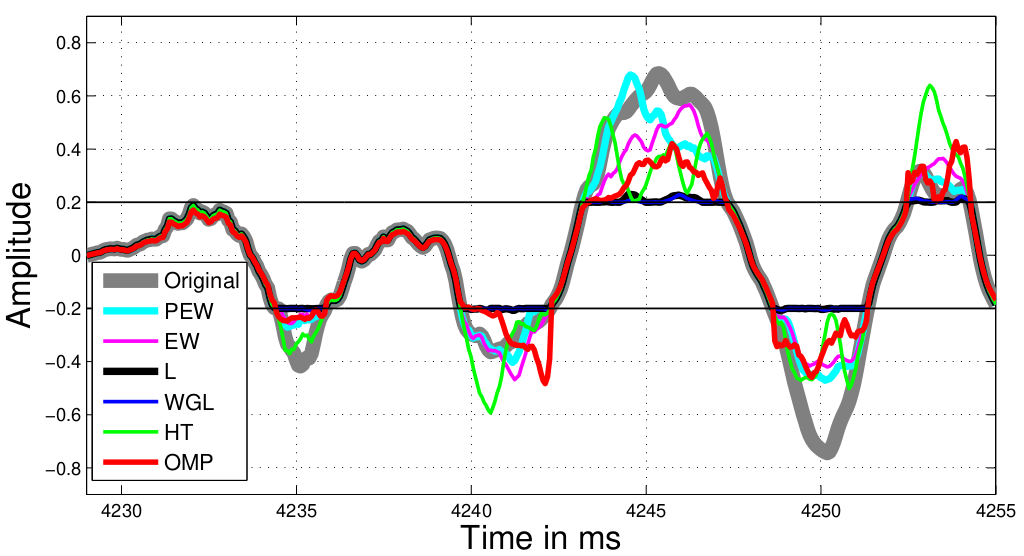
\includegraphics[width=0.48\textwidth]{figures/courb.png}
  \end{center}
  \caption{Declipped signal ($\theta^{clip} = 0.2$) using the Lasso, WGL, EW, PEW, HT, and OMP operators \cite{gaultier:tel-02148598}}
  \label{fig:Df}
\end{wrapfigure}
The autors diclipped same audio signal (speech and music).
The figure \ref{fig:Df} shows the results of a signal with a clipping level $\theta^{clip} = 0.2$ using the different estimators. In the time domain, it turns out that the operators (P)EW , HT and OMP give much better estimates than the (WG)L. OMP appears to produce too many oscillations on high-frequency, while HT occasionally exceeds the original amplitude values.

In the figure \ref{fig:f}, all operators are improving the $SNR_m$. However, Lasso and WGL seem to be the weakest overall. This confirms the results of Figure \ref{fig:Df}.
\begin{figure}[ht!]
    \centering
    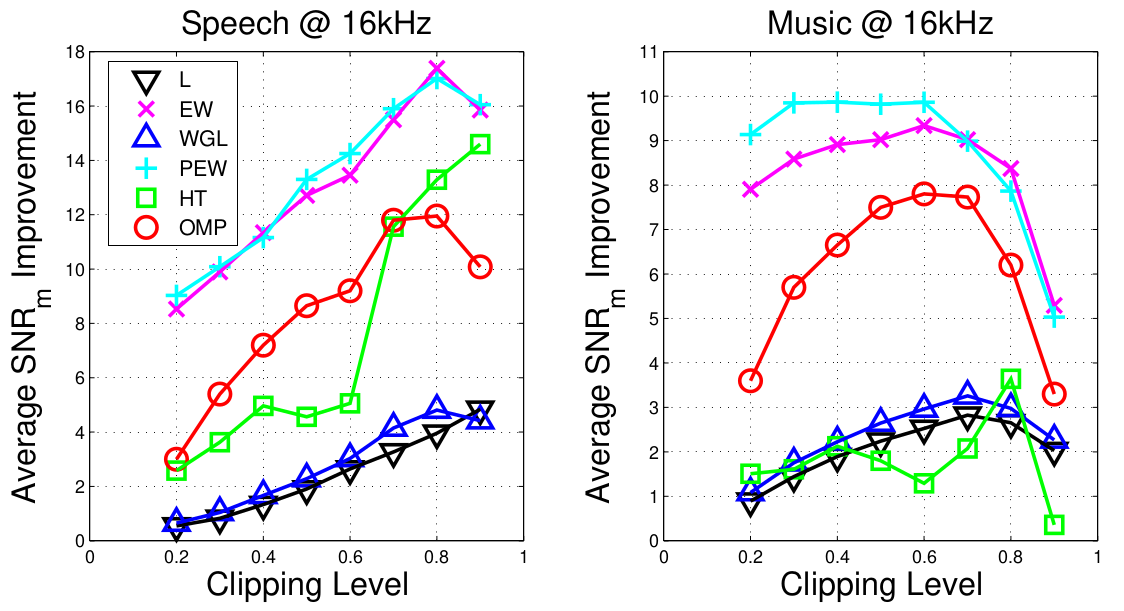
\includegraphics[scale=0.3]{figures/sol.png}
    \caption{The improvement
of $SNR_m$ as a function of clipping level. \cite{gaultier:tel-02148598}}
    \label{fig:f}
\end{figure}
The experiments in \ref{fig:Df} \ref{fig:f} shows that only EW and PEW are well-performing out of the four choices, and they outperform the OMP approache.\\
\section{Implementation}
In the literature there are several toolbox that implement the state of the art declipping techniques. The authors of the paper \cite{záviška2020survey} carried out an in-depth survey to study the different approaches of audio declipping, as well as a comparison between different methods. the authors of \cite{záviška2020survey} provide a matlab declipping toolbox that contains the following methods : 
\begin{table}[ht!]
\begin{tabular}{|l|l|c|}
\hline
Abbreviation & Full name                                                                       & Reference \\ \hline
\rowcolor{Gray}
            C-OMP & Constrained Orthogonal Matching Pursuit                                         &   \cite{5946407}        \\ \hline
             A-SPADE & Analysis SParse Audio DEclipper                                                &       \cite{DBLP:journals/corr/KiticBG15}    \\ \hline
             \rowcolor{Gray}
             S-SPADE& Synthesis SParse Audio DEclipper                                                &   \cite{8682348}        \\ \hline
             ${l}$1 CP& ${l}$1-minimization using Chambolle–Pock (analysis)                                 &   \cite{záviška2020survey}        \\ \hline
             \rowcolor{Gray}
             ${l}$1 DR& ${l}$1-minimization using Douglas–Rachford (synthesis)                              &         \cite{articlve}  \\ \hline
             R${l}$1CC CP& Reweighted ${l}$1-min. with Clipping Constraints using Chambolle–Pock (analysis)    &    \cite{záviška2020survey}       \\ \hline
             \rowcolor{Gray}
              R${l}$1CC DR& Reweighted ${l}$1-min. with Clipping Constraints using Douglas–Rachford (synthesis) &        \cite{DBLP:journals/corr/abs-1110-5063}   \\ \hline
             SS EW& Social Sparsity with Empirical Wiener                                           &     \cite{gaultier:tel-02148598}      \\ \hline
             \rowcolor{Gray}
             SS PEW& Social Sparsity with Persistent Empirical Wiener                                &    \cite{gaultier:tel-02148598}       \\ \hline
CSL1        & Compressed Sensing method minimizing ${l}$1-norm                                    &       \cite{6600777}    \\ \hline
\rowcolor{Gray}
PWCSL1      & Perceptual Compressed Sensing method minimizing ${l}$1-norm                         &       \cite{6600777}     \\ \hline
PWCSL1        & Parabola-Weighted Compressed Sensing method minimizing ${l}$1-norm                  &       \cite{záviška2020survey}    \\ \hline
\rowcolor{Gray}
PW${l}$1 CP       & Parabola-Weighted ${l}$1-minimization using Chambolle–Pock (analysis)               &      \cite{záviška2020survey}     \\ \hline
PW${l}$1 DR      & Parabola-Weighted ${l}$1-minimization using Douglas–Rachford (synthesis)            &       \cite{Zaviska_2019}    \\ \hline
\rowcolor{Gray}
DL           & Dictionary Learning approach                                                    &     \cite{10.1007/978-3-319-93764-9_41}      \\ \hline
NMF          & Nonnegative Matrix Factorization                                                &      \cite{7336948}     \\ \hline
\rowcolor{Gray}
Janssen      & Janssen method for inpainting                                                   &    \cite{1164824}       \\ \hline
\end{tabular}
\end{table}

In the paper the authors compare this methods according to several metrics, for example Signal-to-Distortion Ratio (SDR). the SDR evaluate the physical quality of restoration.
\begin{definition}
The SDR for two signals u and v is defined as:$$
\operatorname{SDR}(\mathbf{u}, \mathbf{v})=20 \log _{10} \frac{\|\mathbf{u}\|_{2}}{\|\mathbf{u}-\mathbf{v}\|_{2}}
$$
\end{definition}
\begin{warn}
The evaluation of  the SDR on the whole signal may penalize the
approaches that produce signals inconsistent in the reliable part.
\end{warn}
To bypass this problem, in \cite{gaultier:tel-02148598} the SDR is computed on the clipped part only. So for a clipped signal y and its estimation $\hat{y}$, SDR is computed as:
$$
\operatorname{SDR}_{c}(\mathbf{y}, \hat{\mathbf{y}})=20 \log _{10} \frac{\left\|\mathrm{M}^{c} y\right\|_{2}}{\left\|\mathrm{M}^{c}(y-\hat{y})\right\|_{2}}
$$
Then the difference between the SDR of the restored and the clipped signal is defined as:
$$\Delta \mathrm{SDR}_{\mathrm{c}}=\operatorname{SDR}_{\mathrm{c}}(\mathrm{y}, \hat{\mathrm{y}})-\operatorname{SDR}_{\mathrm{c}}(\mathrm{y}, \mathrm{s})$$

According to the bar graphs \ref{vdd} the Social Sparsity with Persistent Empirical Wiener method is the most efficient in terms of SDR. For a more detailed comparison check out \cite{záviška2020survey}.

\begin{figure}[ht!]
    \centering
    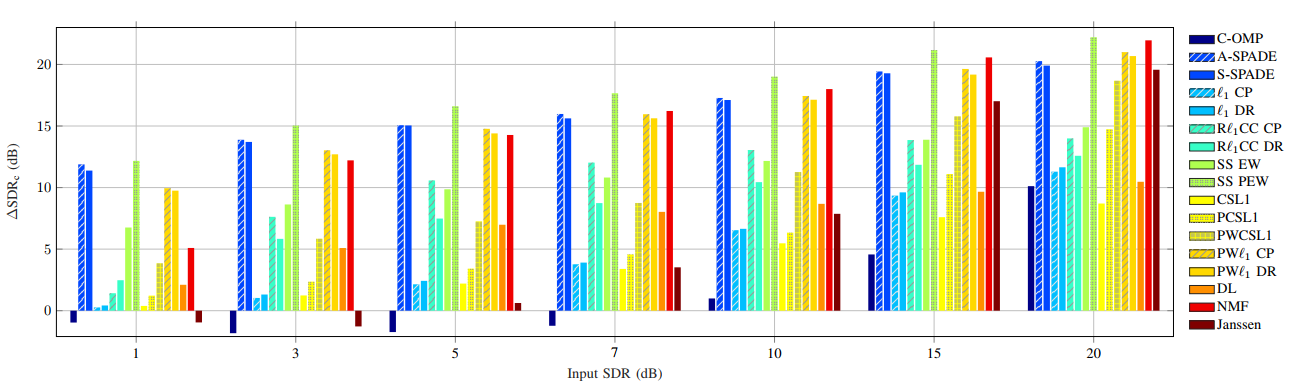
\includegraphics[scale=0.6]{figures/vd.PNG}
    \caption{Average $\Delta SDR_c$ results. \cite{záviška2020survey}}
    \label{vdd}
\end{figure}
The audio declipping toolbox is used to declipped some audio:\\
\textbf{Social Sparsity with Empirical Wiener method:}\\
The Social Sparsity with Empirical Wiener method is tested on a "a08\_violin" audio with the following settings (\ref{function}). the figure \ref{c} show the result of the declipping.\\
\textbf{Output of SS EW}
\begin{itemize}
    \item Result obtained in 1357.491 seconds.
    \item SDR of the clipped signal is 7.000 dB.
    \item SDR of the reconstructed signal is 14.867 dB.
    \item SDR improvement is 7.867 dB.
\end{itemize}

 \lstset{
    language=Matlab,
    tabsize=3,
    %frame=lines,
    caption=settings,
    label=function,
    frame=shadowbox,
    rulesepcolor=\color{gray},
    xleftmargin=20pt,
    framexleftmargin=15pt,
    keywordstyle=\color{blue}\bf,
    commentstyle=\color{blue},
    stringstyle=\color{red},
    numbers=left,
    numberstyle=\tiny,
    numbersep=5pt,
    breaklines=true,
    showstringspaces=false,
    basicstyle=\footnotesize,
    emph={food,name,price},emphstyle={\color{magenta}}}
\begin{lstlisting}[language=Matlab]
% input SDR of the clipped signal
inputSDR = 7;    % set the input SDR value

% DGT parameters
wtype = 'hann';  % window type
w = 8192;        % window length
a = w / 4;       % window shift
M = 2*8192;      % number of frequency channels

% set shrinkage operator
shrinkage = 'EW'; % 'L', 'WGL', 'EW', 'PEW';
number_lambdas = 20;
inner_iterations = 500;
\end{lstlisting}
\begin{figure}[ht!]
    \centering
    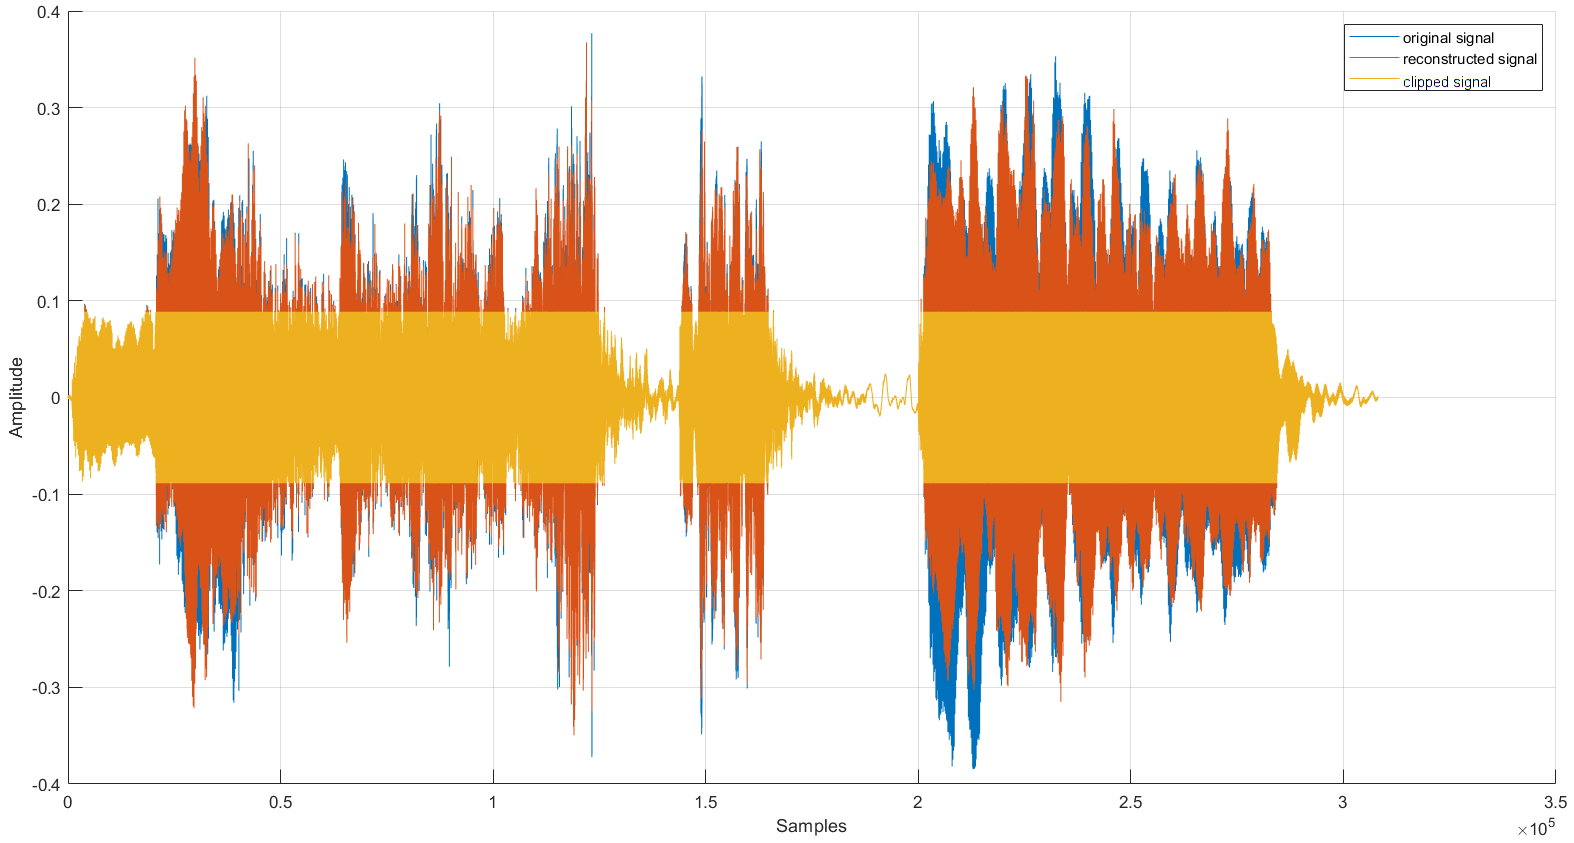
\includegraphics[scale=0.3]{figures/courbe.png}
    \caption{Audio declipping Social according to Social Sparsity with Empirical Wiener}
    \label{c}
\end{figure}
\textbf{Social Sparsity with Persistent Empirical Wiener method:}\\
 the figure \ref{PEW} show the result of the declipping.\\
\textbf{Output of SS PEW}
\begin{itemize}
    \item Result obtained in 1581.076 seconds.
    \item SDR of the clipped signal is 7.000 dB.
    \item SDR of the reconstructed signal is 19.702 dB.
    \item SDR improvement is 12.702 dB.
\end{itemize}

\begin{figure}[ht!]
    \centering
    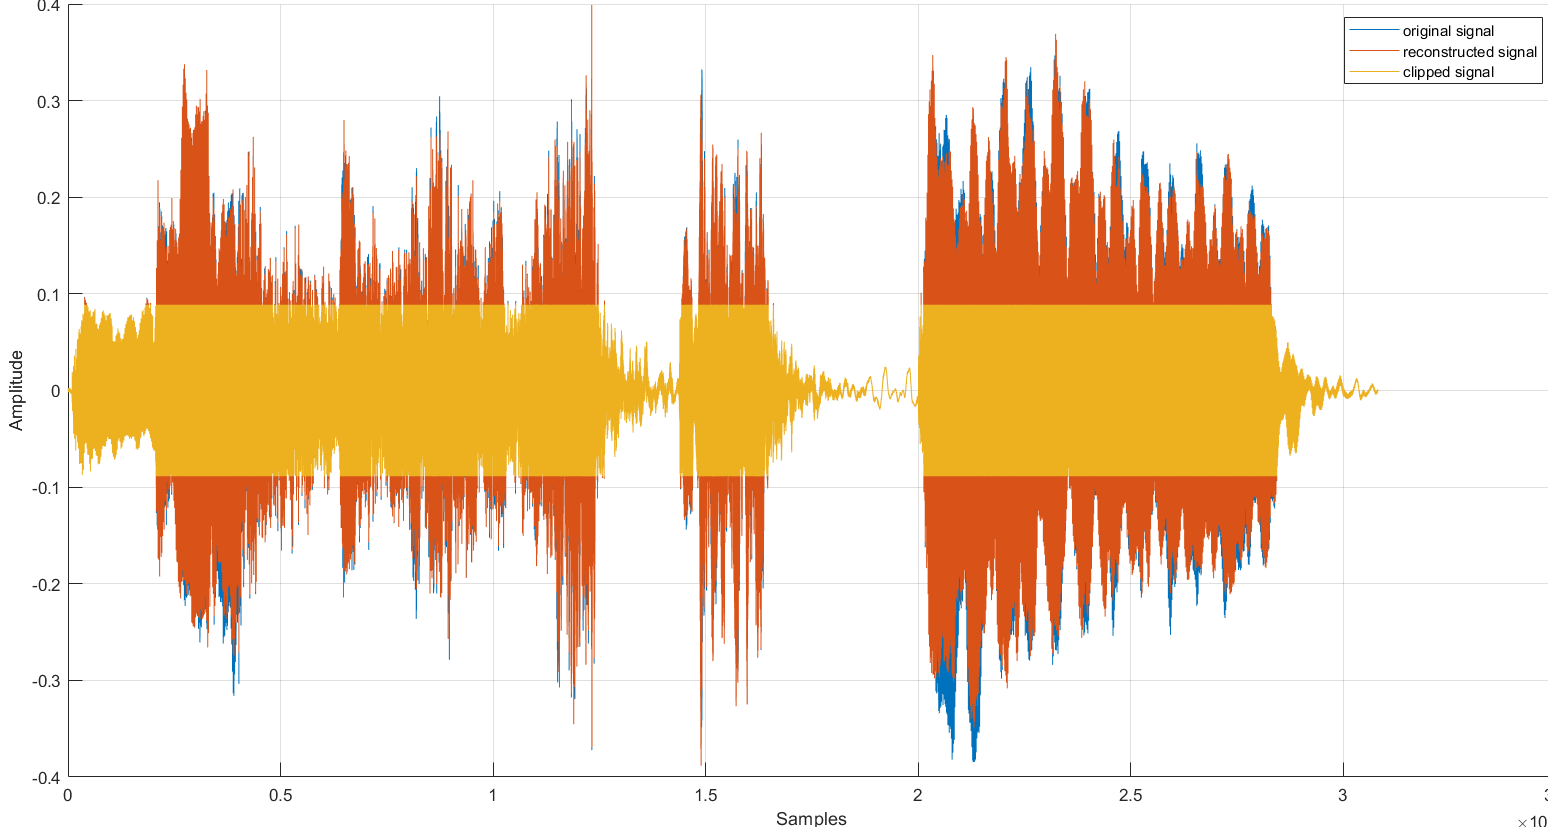
\includegraphics[scale=0.3]{figures/PEW.png}
    \caption{Audio declipping Social according to Social Sparsity with Empirical Wiener}
    \label{PEW}
\end{figure}
\section{Conclusion}
Several techniques have been developed in order to attempt the reversal of a clipped signal.
The article \cite{gaultier:tel-02148598} provides a new approach that outperforms other methods in terms of SDR according to \cite{záviška2020survey}. More precisely The Persistent Empirical Wiener (PEW) operator is used for audio declipping using synthesis social sparsity.
\printbibliography
\end{document}
